\item Use D'Alembert's formula to show the parallelogram property of the wave equation mentioned in class.
\bigbreak
%_____________________________________________________________________________%

\begin{center}
  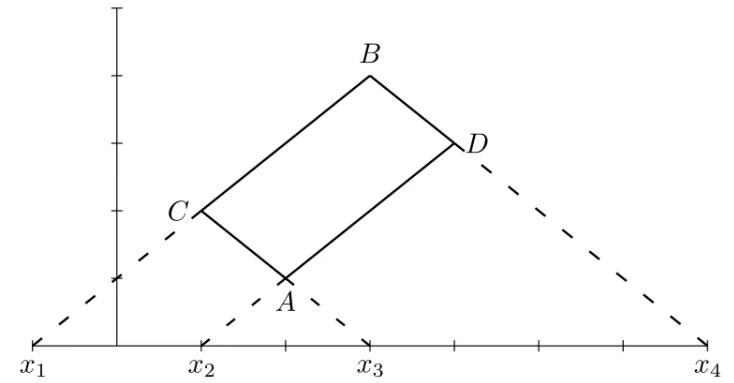
\includegraphics[height=8cm]{1}
\end{center}
%
\begin{align}
  u(A) + u(B) & = u(C) + u(D)
\end{align}

Note that our slope depends on $c$.
Now, let us consider D'Alembert's Formula:
%
\begin{align}
  \frac{1}{2}[f(x + t) + f(x - t)] + \frac{1}{2} \int^{x + t}_{x - t} g(y)
  \text dy
\end{align}

Now, let us consider using D'Alembert's Formula to generate the following equations:
%
\begin{align}
  u(A) & = \frac{1}{2} [f(x_2) + f(x_3)] + \frac{1}{2c} \int^{x_3}_{x_2} g(y) \text\ dy\\
  u(B) & = \frac{1}{2} [f(x_1) + f(x_4)] + \frac{1}{2c} \int^{x_4}_{x_1} g(y) \text\ dy\\
  u(C) & = \frac{1}{2} [f(x_1) + f(x_3)] + \frac{1}{2c} \int^{x_3}_{x_1} g(y) \text\ dy\\
  u(D) & = \frac{1}{2} [f(x_2) + f(x_4)] + \frac{1}{2c} \int^{x_4}_{x_2} g(y) \text\ dy
\end{align}

From here, let us evaluate $u(A) + u(B)$ and $u(C) + u(D)$
%
\begin{align}
  u(A) + u(B) & =
  \frac{1}{2} [f(x_2) + f(x_3)] + \frac{1}{2c} \int^{x_3}_{x_2} g(y) \text\ dy +
  \frac{1}{2} [f(x_1) + f(x_4)] + \frac{1}{2c} \int^{x_4}_{x_1} g(y) \text\ dy\\
  & =
  \frac{1}{2} \left( f(x_1) + f(x_4) + f(x_2) + f(x_3) +
  \frac{1}{c}\left[
  \int^{x_4}_{x_1} g(y) \text dy + \int^{x_3}_{x_2} g(y) \text dy
  \right]\right)
\end{align}

Next, evaluate $u(C) + u(D)$:
%
\begin{align}
  u(C) + u(D) & =
  \frac{1}{2} [f(x_1) + f(x_3)] + \frac{1}{2c} \int^{x_3}_{x_1} g(y) \text\ dy  +
  \frac{1}{2} [f(x_2) + f(x_4)] + \frac{1}{2c} \int^{x_4}_{x_2} g(y) \text\ dy \\
  & = \frac{1}{2}
  \left(
  f(x_1) + f(x_3) + f(x_2) + f(x_4) + \frac{1}{c}
  \left[
  \int^{x_3}_{x_1} g(y) \text\ dy +
  \int^{x_4}_{x_2} g(y) \text\ dy
  \right]
  \right)
\end{align}

If we analyze the regions of our integral, we can observe the interval length of the integral for $u(A) + u(B)$ spans over 10 units. In addition, $u(C) + u(D)$ also spans over 10 intervals once again. Here, both intervals are equal.
Therefore,
%
\begin{align}
  u(A) + u(B) & = u(C) + u(D)
\end{align}
